\documentclass[conference]{IEEEtran}
\IEEEoverridecommandlockouts
% The preceding line is only needed to identify funding in the first footnote. If that is unneeded, please comment it out.
%Template version as of 6/27/2024

\usepackage{cite}
\usepackage{amsmath,amssymb,amsfonts}
\usepackage{algorithmic}
\usepackage{graphicx}
\usepackage{minted}
% \usepackage{caption}
% \captionsetup{font=small}
\usepackage{xcolor} % to access the named colour LightGray
\definecolor{LightGray}{gray}{0.9}

\def\BibTeX{{\rm B\kern-.05em{\sc i\kern-.025em b}\kern-.08em
    T\kern-.1667em\lower.7ex\hbox{E}\kern-.125emX}}
\begin{document}

\title{Rules}

\author{  
  \IEEEauthorblockN{
  }
}  

\maketitle

\section{Overview}
\label{sec:overview}
This game is a tactical dueling card game for two to six players.
The objective is to battle for control of various locations by summoning your creatures to defend them.
The player who maintains the most power over these locations emerges as the winner. 
However, strategy is key, as each location has limited space, requiring careful planning when summoning your creatures.

\section{Setup}
\label{sec:setup}
Each player must bring their own deck of 15 unique cards.
Shuffle each other's decks before playing.
Players start with 4 cards in their hand.
Choose the starting player at random.
Starting with the player going first, each player has the option to "mulligan" once.
To mulligan, each player may put any number of cards from their hand at the bottom of their deck, then draw that many cards.

Play proceeds clockwise.
A player's turn consists of the following steps:
\begin{enumerate}
    \item Drawing a card
    \item Getting a mana crystal
    \item Playing cards (optional)
  \end{enumerate}
At the start of their turn, a player draws a card from their deck and takes a new mana crystal of a color of their choice. 
The available colors are red, green, and blue.
The maximum amount of mana crystals a player can have is seven.
The player may then play cards from their hand, spending the required mana.
The card shown in Figure \ref{fig:CreatureCardExample} costs four mana in total: Two mana of any color, one red mana, and one blue mana.
Spent mana crystals are kept, but you can only use them again in your next turn.
Most cards are creature cards, which have an effect and power and must be played on a location.

\begin{figure}[ht]
  \centerline{
\includegraphics[width=0.30\textwidth]{images/Volatile Alchemist.png}}
  \caption{Creature card.}
  \label{fig:CreatureCardExample}
\end{figure}

Locations have a maximum number of creatures that can be played on them.
When you play creatures on a location, play them face up on a stack.
Each player has their own creature stack.
Stack the cards so that the creatures powers are always visible.
The player with the highest sum of creature powers on a location wins it.
After each round, determine who is currently winning at most of the locations.
Be aware that some locations might count more; for example, in a two-player game, the center location is worth $1.5\times$ compared to one of the outside locations.
The player currently winning the most locations gains a victory point and starts the new round.
In case of a tie, the player with the highest total power wins.
If it is still a tie, the player who started the last round starts the new round.
The first player to earn four victory points wins the game.
The game ends after 7 rounds.
If no player has four victory points by the end, the player who won the last round wins the game.

The number of locations and who can play at them varies with number of players:

\section{Two Player Rules}
\label{sec:twoplayer}

\begin{figure}[ht]
    \centerline{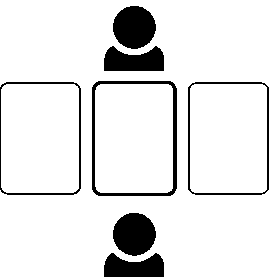
\includegraphics[width=0.1\textwidth]{images/2player.pdf}}
    \caption{Setup for a two-player game. The highlighted center location is worth more than the outside locations. 7 creature cards can be played at each of the locations.}
    \label{fig:TwoPlayerSetup}
\end{figure}
Figure \ref{fig:TwoPlayerSetup} illustrates the location setup for a two-player game.
Each location can hold up to seven creature cards.
The center location is worth more than the outer locations.
If the players decide to play with location cards (see section \ref{subsec:location}), the outside locations are replaced by the players' location cards at the start of the game.

\section{Multiplayer Rules}
\label{sec:multiplayer}
\subsection{Free for All}
\label{subsec:ffa}

In Free for All (FFA) games, every player plays for their own victory.
The outside locations are only accessible by their two closest players, while the center locations are accessible to all.
Cards of a player can only be played on a location accessible by that player and may not be moved to any location inaccessible to them.
Card effects targeting cards on inaccessible locations are allowed.
At every location, $X\times3 + 1$ creatures can be played at maximum, where $X$ is the number of players able to play on that location.

\begin{figure}[ht]
  \centerline{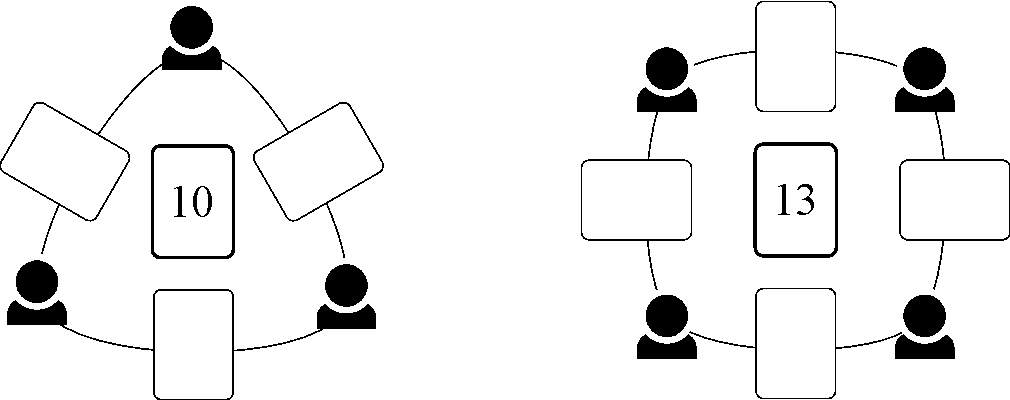
\includegraphics[width=0.4\textwidth]{images/ffa_small.pdf}}
  \caption{Setup for a three and four-player FFA game. The number shows the available creature slots of the more valuable center location. The outside locations have seven creature slots.}
  \label{fig:3playerSetup}
\end{figure}
\begin{figure}[ht]
  \centerline{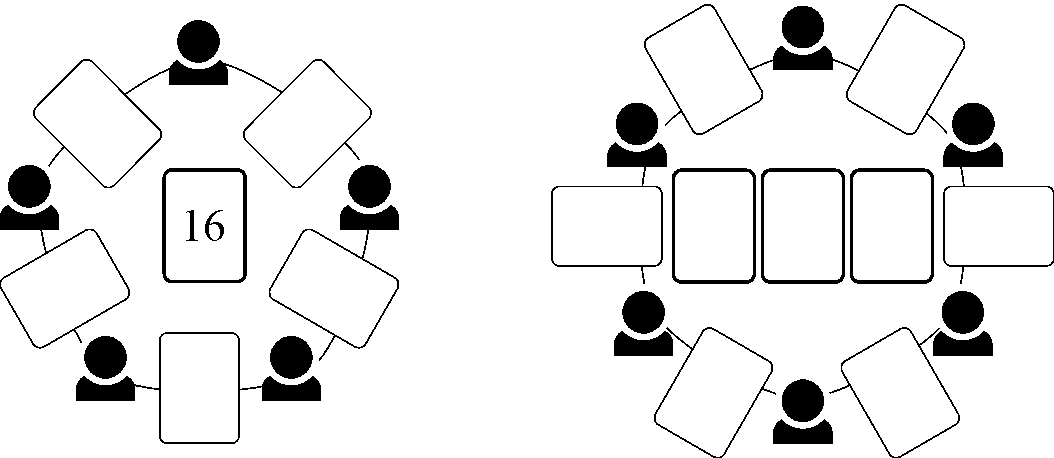
\includegraphics[width=0.4\textwidth]{images/ffa_big.pdf}}
  \caption{Setup for a five and six-player FFA game. The number shows the available creature slots. The center location(s) are worth more. Locations without a number have seven creature slots.}
  \label{fig:4playerSetup}
\end{figure}

\subsection{Team Games}
\label{subsec:team}
\begin{figure}[hb]
  \centerline{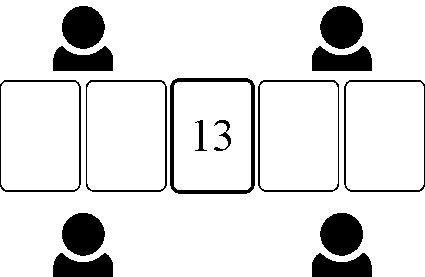
\includegraphics[height=0.1\textwidth]{images/2v2.pdf}}
  \caption{Setup for a 2vs2 team game. The highlighted center location is playable by all players and is worth more.}
  \label{fig:2v2Setup}
\end{figure}
\begin{figure}[hb]
  \centerline{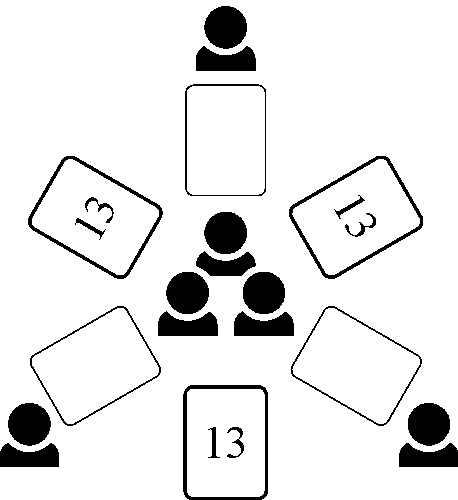
\includegraphics[width=0.15\textwidth]{images/3v3.pdf}}
  \caption{Setup for a 3vs3 team game. The locations without a number are playable by the two players directly sitting in front of them. The valuable locations with 13 creature slots are playable by the four closest players.}
  \label{fig:3v3Setup}
\end{figure}
\begin{figure}[ht]
  \centerline{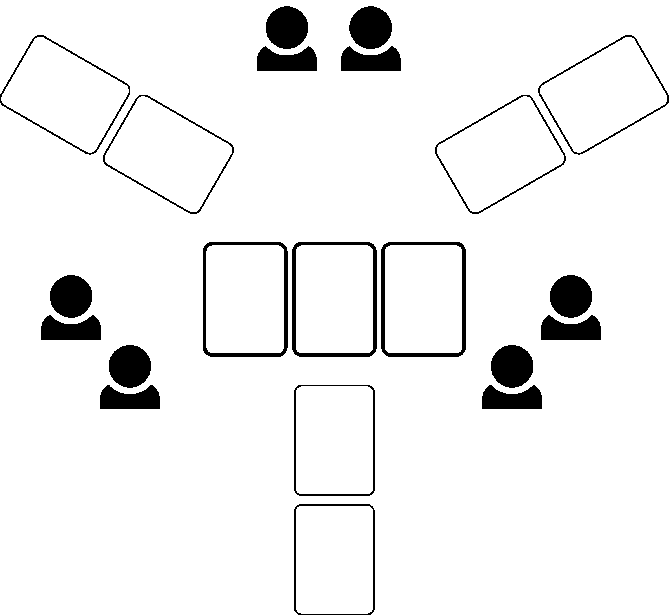
\includegraphics[width=0.25\textwidth]{images/2v2v2.pdf}}
  \caption{Setup for a 2vs2vs2 team game. The outside locations are playable by two players. The valuable center locations are accessible to all.}
  \label{fig:3v3Setup}
\end{figure}
The game can also be played 2vs2, 3vs3 or 2vs2vs2.
The players of one team must sit on the same side of the table and face their opposing players.
For 2vs2, there are five locations.
The outside locations can only be played by the two players closest to them on that side.
The center location can be played by all players and has slots for 13 creature cards.
For 3vs3, there are six locations.
The players can only play on the three locations closest to them (see Figure \ref{fig:3v3Setup}).


\section{Keywords and Terminology}
\label{sec:keywords}
\textbf{Graveyard} A face up pile of cards with all your destroyed or discarded cards. Every player has their own graveyard.\\
\textbf{Additional cost:} Must be paid to play the card.\\
\textbf{On Play:} Triggers when you play this creature from your hand. Entering the battlefield through other means like revive do not trigger this.\\
\textbf{Friendly creature} A creature under your control.\\
\textbf{Destroy a creature} Select a creature and put it into their owner's graveyard.\\
\textbf{Discard a card} Select a card in your hand and put it in your graveyard.\\
\textbf{Move a creature} Select a creature and move it on top of the creature stack of another location accessible to the creature's owner.\\
\textbf{Return a creature} Select a creature in play and return it to their owner's hand.\\
\textbf{Revive a creature} Select a creature in your graveyard and place it on top of your creature stack of a location accessible to you.\\
\textbf{Get an extra mana crystal} Get an extra mana crystal. You can use it immediately.\\
\textbf{Destroy} Put an enemy creature into their owner's graveyard.\\
\textbf{On Draw:} Triggers when you draw this creature from your deck.\\
\textbf{On Destruction:} Triggers when this creature is destroyed.\\
\textbf{On Discard:} Triggers when this creature is discarded.\\
\textbf{On Return:} Triggers when this creature is returned from the battlefield or graveyard to your hand.\\
\textbf{On Revive:} Triggers when this creature is revived.\\
\textbf{On Move:} Triggers when this creature is moved.\\
\textbf{While on top} Is only active when this creature is the topmost creature on your creature stack.\\
\textbf{Gain control of an enemy creature} Select an enemy creature and put it on top of your creature stack at that same location.\\
\textbf{Gift a creature to an opponent} Select a friendly creature and put it on top of one of your opponent's creature stacks at that same location.\\

\section{Advanced rules}
\subsection{Side-boarding}
\label{subsec:sideboard}
In best-of-three formats, you may bring an extra 15-card deck in addition to the main deck.
Between the games, you may modify your main deck by up to 5 cards from your extra deck.
Location cards, hero cards, and fusion creature cards count towards this extra deck, but cannot be swapped into the main deck.

\subsection{Hero Cards}
\label{subsec:hero}
You may bring a single hero card in your extra deck.
To use the hero's ability, you must pay one victory point and the mana cost on the hero card.

\subsection{Location Cards}
\label{subsec:location}
You may bring up to five different location cards. 
At the start of the game select one of them at random and put it on the outside location on your left.

\section*{Acknowledgment}

Thank you to my lovely play testers: 
Aki, Ina, Volkmar, Myriam, Charlotta, Julia, Niko, Maxi, Julia, Karl, Lukas, Thai, David, Andi
\vspace{12pt}

\end{document}
